% XeLaTeX document
\documentclass[12pt,a4paper]{article}

% Редактируем: конфигурация, личные настройки: имя, название предмета и пр. для титульной страницы и метаданных документа здесь
\newcommand{\university}{Московский государственный университет имени М. В. Ломоносова}
\newcommand{\faculty}{Экономический факультет}
%\newcommand{\department}{Высшая школа прикладной математики и вычислительной физики}
\newcommand{\city}{Москва}
\newcommand{\num}{ №1}
\newcommand{\docname}{Анализ монетарной политики ЦБ РФ}
\newcommand{\subject}{Введение в экономику}
%\newcommand{\tutorname}{С. Г. Попов}
\newcommand{\studentname}{Михайлов Д.Р. \,Матевосова А.М. \,Зудин А.С}
\newcommand{\group}{э101}

% Не редактируем: используемые пакеты
% настройка кодировки, шрифтов и русского языка
\usepackage{fontspec}
\usepackage{polyglossia}

% рабочие ссылки в документе
\usepackage{hyperref}

% графика
\usepackage{graphicx}
\usepackage{tikz}

% поворот страницы
\usepackage{pdflscape}

% качественные листинги кода
\usepackage{minted}
\usepackage{listings}
\usepackage{lstfiracode}

% отключение копирования номеров строк из листинга, работает не во всех просмотрщиках (в Adobe Reader работает)
\usepackage{accsupp}
\newcommand\emptyaccsupp[1]{\BeginAccSupp{ActualText={}}#1\EndAccSupp{}}
\let\theHFancyVerbLine\theFancyVerbLine
\def\theFancyVerbLine{\rmfamily\tiny\emptyaccsupp{\arabic{FancyVerbLine}}}

% библиография
\bibliographystyle{templates/gost-numeric.bbx}
\usepackage{csquotes}
\usepackage[parentracker=true,backend=biber,hyperref=true,bibencoding=utf8,style=numeric-comp,language=auto,autolang=other,citestyle=gost-numeric,defernumbers=true,bibstyle=gost-numeric,sorting=ntvy]{biblatex}

% установка полей
\usepackage{geometry}

% нумерация картинок по секциям
\usepackage{chngcntr}

% дополнительные команды для таблиц
\usepackage{booktabs}

% для заголовков
\usepackage{caption}
\usepackage{titlesec}
\usepackage[dotinlabels]{titletoc}

% разное для математики
\usepackage{amsmath, amsfonts, amssymb, amsthm, mathtools}

% водяной знак на документе, см. main.tex
\usepackage[printwatermark]{xwatermark}

\usepackage{tikz} %Работа с графикой
\usepackage{pgfplots}
\pgfplotsset{compat=newest}
\usepackage{pgfplotstable}

\usepgfplotslibrary{dateplot}%Пакет для графиков с датой

\usepackage{attachfile}%Пакет для приложения файла


% Не редактируем: параметры используемых пакетов и не только
% настройки polyglossia
\setdefaultlanguage{russian}
\setotherlanguage{english}

% локализация
\addto\captionsrussian{
	\renewcommand{\figurename}{Рисунок}%
	\renewcommand{\partname}{Глава}
	\renewcommand{\contentsname}{\centerline{Содержание}}
	\renewcommand{\listingscaption}{Листинг}
}

% основной шрифт документа
\setmainfont{CMU Serif}
\newfontfamily\cyrillicfont{CMU Serif}[Script=Cyrillic]

% перечень использованных источников
\addbibresource{refs.bib}

% настройка полей

\geometry{bottom=2.5cm}
\geometry{left=2cm}
\geometry{right=2cm}
\geometry{top=2cm}
\geometry{bindingoffset=0cm}

% настройка ссылок и метаданных документа
\hypersetup{unicode=true,colorlinks=true,linkcolor=black,citecolor=blue,filecolor=magenta,urlcolor=cyan,
	pdftitle={\docname},
	pdfauthor={\studentname},
	pdfsubject={\subject},
	pdfcreator={\studentname},
	pdfproducer={Overleaf},
	pdfkeywords={\subject}
}

% настройка подсветки кода и окружения для листингов
\usemintedstyle{colorful}
\newenvironment{code}{\captionsetup{type=listing}}{}

% шрифт для листингов с лигатурами
\setmonofont{FiraCode-Regular.otf}[
	SizeFeatures={Size=10},
	Path = templates/,
	Contextuals=Alternate
]

% оформления подписи рисунка
\captionsetup[figure]{labelsep = period}

% подпись таблицы
\DeclareCaptionFormat{hfillstart}{\hfill#1#2#3\par}
\captionsetup[table]{format=hfillstart,labelsep=newline,justification=centering,skip=-10pt,textfont=bf}

% путь к каталогу с рисунками
\graphicspath{{fig/}}

% Внесение titlepage в учёт счётчика страниц
\makeatletter
\renewenvironment{titlepage} {
	\thispagestyle{empty}
}
\makeatother

\counterwithin{figure}{section}
\counterwithin{table}{section}

\titlelabel{\thetitle.\quad}

% для удобного конспектирования математики
\mathtoolsset{showonlyrefs=true}
\theoremstyle{plain}
\newtheorem{theorem}{Теорема}[section]
\newtheorem{proposition}[theorem]{Утверждение}
\theoremstyle{definition}
\newtheorem{corollary}{Следствие}[theorem]
\newtheorem{problem}{Задача}[section]
\theoremstyle{remark}
\newtheorem*{nonum}{Решение}

% настоящее матожидание
\newcommand{\MExpect}{\mathsf{M}}

% объявили оператор!
\DeclareMathOperator{\sgn}{\mathop{sgn}}

% перенос знаков в формулах (по Львовскому)
\newcommand*{\hm}[1]{#1\nobreak\discretionary{} {\hbox{$\mathsurround=0pt #1$}}{}}


% водяной знак для обозначения статуса документа
%\newwatermark[allpages,color=red!15,angle=45,scale=3,xpos=0,ypos=0]{IN  PROGRESS}
\begin{document}
% Не редактируем: Титульная страница (формируется автоматически из заданной конфигурации)
\newgeometry{bottom=2cm, left=2cm, right=2cm, top= 2cm, bindingoffset=0cm}

\begin{titlepage}	% начало титульной страницы

	\begin{center}		% выравнивание по центру
  %\textcolor{white}{  }\\[6cm]
		\large \university \\
		\large \faculty \\[5cm]
		%\large \department \\[6cm])
		% название института, затем отступ 6см

		%(\huge \subject \\[0.5cm] % название работы, затем отступ 0,5см
		%\large \docname  \\[5.1cm])
		% \large Тема работы\\[5cm]
        
        
        %\huge \subject \\[0.5cm]  %название работы, затем отступ 0,5см
		\huge \docname  \\[5.1cm]
		
	\end{center}


	
%(\begin{flushright} % выравнивание по правому краю
%		\begin{minipage}{0.25\textwidth} % врезка в половину ширины текста
%			\begin{flushleft} % выровнять её содержимое по левому краю
%
%				\large\textbf{Работу выполнил:}\\
%				\large \studentname \\
%				\large {Группа:} \group \\
%
%				\large \textbf{Преподаватель:}\\
%
%			\end{flushleft}
%		\end{minipage}
%	\end{flushright})
\begin{center}
				\large \studentname \\
				\large {Группа:} \group \\ [0.5cm]

				%\large \textbf{Преподаватель:}\\
				%\large \tutorname
                
                
		        %\large \faculty \\
		        %\large \university \\
	        	%\large \department			
\end{center}
	

	\vfill % заполнить всё доступное ниже пространство

	\begin{center}
	%	\large \city \\
		\large \the\year % вывести дату
	\end{center} % закончить выравнивание по центру

\end{titlepage} % конец титульной страницы
\restoregeometry
\vfill % заполнить всё доступное ниже пространство


% Не редактируем: Страница содержания (формируется автоматически из section, subsection и пр., указанных в content.tex)
% Содержание
\tableofcontents
\newpage



% Редактируем: всё остальное: вступление, др. этапы, заключение, приложение
\section{Введение}
\hypersetup{unicode=true,colorlinks=true,linkcolor=red,citecolor=blue,filecolor=magenta,urlcolor=cyan,
	pdftitle={\docname},
	pdfauthor={\studentname},
	pdfsubject={\subject},
	pdfcreator={\studentname},
	pdfproducer={Overleaf},
	pdfkeywords={\subject}
}
\noindent
В данной работе перед нами стояла задача рассмотреть динамику инфляции и ключевой ставки процента в России за период с 2014 года по настоящее время. Мы начали выполнение задания со сбора данных о соответствующих показателях за разные промежутки времени и с построения графиков. Они показали нам, что между величинами есть связь, которую мы смогли объяснить макроэкономической теорией. В работе представлен анализ денежной политики, проводимой в России. Он сопоставлен с периодами роста и понижения ключевой ставки процента; на основе исследования отчётов Центрального Банка приведены причины, по которым такая политика была необходима. В дополнение на языке программирования R нами был написан интерактивный график\footnote{\href{https://cloud.mail.ru/public/Ghzc/5BbkoCXiv/}{Интерактивный график}}, иллюстрирующий динамику ключевой ставки с комментариями о причинах её изменений. Далее приведено исследование динамики уровня инфляции в России: графики и их краткое описание. Указано, как изменился уровень ИПЦ в стране в настоящее время по сравнению с переходом Банка России в 2014 году к новому виду монетарной политики – инфляционному таргетированию. В дополнение нами представлен прогноз показателя инфляции за декабрь 2021 года (официальных данных на момент написания работы не было), полученный путём использования моделей ARIMA и SARIMA\footnote{\href{https://colab.research.google.com/drive/1Ushl61tjySwsZcWbtuyYa8YFMHhyUuRv?usp=sharing}{Прогноз уровня инфляции}}.


\newpage

%\begin{itemize}
%	\item Изменить \textbf{config.tex}: имя студента, название предмета и пр. параметры указаны именно там
%	\item Заполнить \textbf{content.tex} - файл, который будет содержать весь текст отчёта, от вступления до заключения.
%	\item Добавить используемую литературу (если есть) в \textbf{refs.bib}. Для удобного поиска источников можно воспользоваться Google Books. Использованные источники можно указывать с помощью команды \textbf{\\cite\{name\_of\_ref\}}


\section{Ключевая ставка}
\subsection{Предисловие}
\noindent
\textit{Ключевая ставка процента} — это основной инструмент Банка России для проведения монетарной политики. Под этот процент коммерческие банки берут кредиты у центрального, изменение этого показателя свидетельствует о проведении стимулирующей (понижение приводит к большему количеству кредитов, а следовательно, денег в обращении) или сдерживающей политики (повышение ставки имеет обратный эффект). Заметим, что стимулирование экономики, вследствие описанного правила, приводит к повышению уровня инфляции, в то время как сдерживание, наоборот, способно понизить его.
\subsection{Анализ динамики ключевой ставки \cite{press_release}}
%\begin{figure}[H]
%   \centering
% 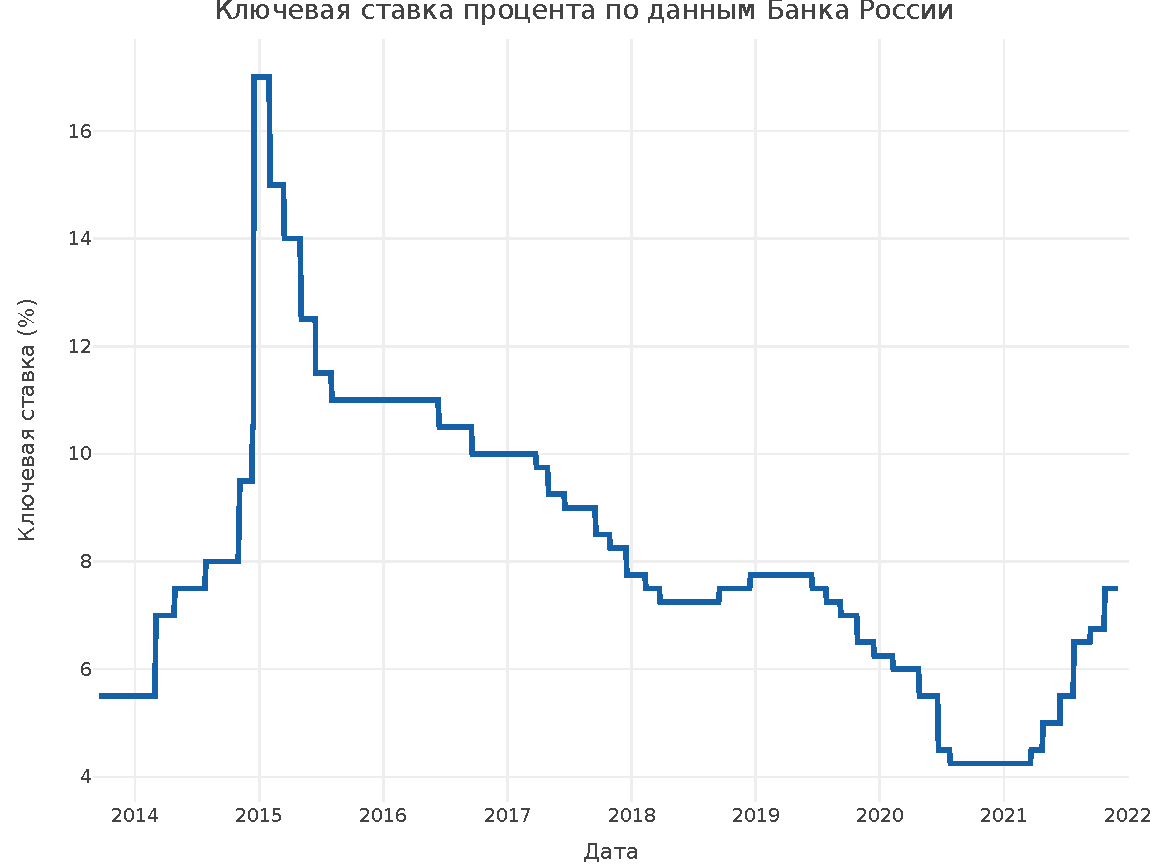
\includegraphics[scale = 0.88]{fig/interestforTEX.pdf}
%    \caption{Ключевая ставка \cite{interest_rate}}
%    \label{fig:int_rate}
%\end{figure}
%grid = both, minor tick num = 1
%\attachfile{fig/interestrate5.html}{\textcolor{blue}{\LaTeX}}

\begin{figure}[H]
\centering
\begin{tikzpicture}[scale=1]
\begin{axis}[thin, date coordinates in=x,xmin=2013-09-10,xmax=2022-01-01, xticklabel style={rotate=0},xtick={2014-01-01,2015-01-01,2016-01-01,2017-01-01,2018-01-01,2019-01-01,2020-01-01,2021-01-01, 2022-01-01},
xticklabel={\year}, ymin = 0, grid, major grid style = {lightgray!40},  width = \linewidth]
\addplot[blue,very thick,] table[x index=0,y index=1,col sep=comma]{fig/Stavka1.txt};
%\legend{Нефть Brent, Нефть WTI}
\end{axis}
\end{tikzpicture}
\caption{Ключевая ставка \cite{interest_rate}}
\end{figure}

\newpage
\subsubsection*{Март 2014 – Январь 2015}
\noindent
\emph{Сдерживающая политика}

\noindent
За десять месяцев ключевая ставка процента выросла с 5,5\% до 17\% годовых. Сначала необходимость повышения ключевой ставки была вызвана желанием предотвратить возникновение инфляционных рисков, но влияние волатильности на финансовых рынках, курсовой динамики и нестабильности внешних условий на потребительские цены оказалось слишком высоким: к концу осени инфляция вдвое превышала таргетируемый уровень и, согласно прогнозам, оставалась бы на таком уровне ещё продолжительное время, что привело к необходимости дальнейшего повышения ключевой ставки. 16 декабря 2014 года ключевую ставку подняли сразу на 6,5\% до её рекордного уровня: причинами стали падение цен на нефть – основной экспортный товар России \footnote{Олег Ицхоки,Ведомости \href{https://www.vedomosti.ru/opinion/articles/2015/01/12/valyutnyj-krizis-20142015-gg}{Валютный кризис 2014-2015 годов}} \cite{CurrencyCrisis}, война на Украине, западные санкции \footnote{РБК  \href{https://www.rbc.ru/economics/09/02/2015/54d7cccf9a79471f9f83f9dd}{Сбили с курса: как война, санкции, нефть и ЦБ уронили рубль}} \cite{War} и, как следствие, обвал рубля и валютный кризис.

\subsubsection*{Январь 2015 – Июль 2015}
\noindent
\emph{Стимулирующая политика (смягчение сдерживающей)}

\noindent
Очень высокое значение ключевой ставки помогало бороться с инфляцией, но появлялись новые серьёзные вызовы для экономики – её охлаждение (существенное замедление экономической активности, а значит и развития всей экономики). Так как баланс рисков был смещён в сторону охлаждения экономики, а инфляционные риски ослабились, было принято решение снижать ключевую ставку: за полгода ключевая ставка постепенно снижалась с 17\% до 11\% годовых.

\subsubsection*{Июль 2015 – Июнь 2016}
\noindent
\emph{Продолжение ведения стимулирующей политики}

\noindent
Почти год ставка сохранялась на уровне 11\% годовых; сначала это была вынужденная мера: увеличивались инфляционные риски, но риски охлаждения экономики оставались существенными. К весне 2016 года совет директоров Банка России начал отмечать позитивные процессы: замедление инфляции, снижение инфляционных ожиданий и приближающийся восстановительный рост экономики.

\subsubsection*{Июнь 2016 – Март 2017}
\noindent
\emph{Стимулирующая политика}

\noindent
В результате описанных изменений ставка была снижена сначала до уровня в 10,5\%, а через три месяца до 10\% годовых. На таком значении она держалась почти 5 месяцев: это требовалось, чтобы закрепить тенденции к стабилизации экономической активности (в начале этого периода она была крайне неустойчивой), снижению инфляции и инфляционных ожиданий.

\subsubsection*{Март 2017 – Март 2018}
\noindent
\emph{Стимулирующая политика}

\noindent
Плавное снижение ключевой ставки с 10\% до 7,25\% годовых: вначале замедление инфляции шло быстрее, чем прогнозировалось, вскоре её значение стало находиться вблизи целевого уровня и ниже, но среднесрочные инфляционные риски сохранялись. В декабре 2017 она составляла 2,5\%, что в совокупности с продлением соглашения об ограничении добычи нефти (это событие также снижало проинфляционные риски) позволило продолжать снижать ставку.

\subsubsection*{Март 2018 – Август 2018}
\noindent
\emph{Продолжение ведения стимулирующей политики}

\noindent
Продолжительный период времени ставка оставалась на уровне 7,25\% годовых, так как инфляция находилась на устойчиво низком уровне, инфляционные ожидания постепенно снижались, как и связанные риски. В середине рассматриваемого периода произошло ослабление рубля на фоне геополитических напряжённостей, что привело к более быстрому приближению уровня роста потребительских цен к установленному таргету Банка России, также Банк России пересмотрел вверх прогноз по инфляции с учётом эффекта от предлагаемого повышения НДС в 2019 году.

\subsubsection*{Сентябрь 2018 – Декабрь 2018}
\noindent
\emph{Сдерживающая политика}

\noindent
Впервые с 2014 года ставка была повышена: сначала до 7,5\%, позже до 7,75\% годовых. Инфляция уже превышала цели Банка России, сохранялась неопределённость относительно дальнейшего развития внешних условий и реакции инфляционных ожиданий на будущее повышение НДС.

\subsubsection*{Декабрь 2018 – Июнь 2019}
\noindent
\emph{Продолжение ведения сдерживающей политики}

\noindent
Длительное время ключевая ставка сохранялась на уровне 7,75\% годовых. Это позволило скомпенсировать вклад повышения НДС в годовые темпы роста потребительских цен, и в апреле инфляция преодолела свой пик, после чего начала замедляться. Краткосрочные инфляционные риски постепенно снижались.

\subsubsection*{Июнь 2019 – Декабрь 2019}
\noindent
\emph{Стимулирующая политика}

\noindent
Ключевая ставка постепенно снижалась до 6,25\%, так как темпы роста российской экономики были ниже ожиданий Банка России, продолжалось замедление инфляции.  Дезинфляционные риски начинали преобладать над проинфляционными в краткосрочном периоде.

\subsubsection*{Декабрь 2019 – Июль 2020}
\noindent
\emph{Стимулирующая политика}

\noindent
Уже более стремительно ставка была понижена до 4,25\% годовых, так как произошло существенное отклонение от прогнозов Банка России: этому поспособствовали распространение пандемии и связанные с ней ограничения, крайне сильное снижение цен на нефть, замедление развития экономики и растущая неопределённость относительно ожиданий. Со временем оказалось, что дезинфляционные факторы играли ещё более значимую роль, чем рассчитывалось.

\subsubsection*{Июль 2020 – Март 2021}
\noindent
\emph{Продолжение ведения стимулирующей политики}

\noindent
Сначала рост цен складывался выше ожиданий Банка Росси: после самоизоляции спрос восстанавливался очень быстро, параллельно наблюдалось ослабление рубля, волатильность на мировых рынках и усиление геополитических рисков. Но прогнозировалось также и серьёзное ухудшение эпидемиологической обстановки, что могло бы сыграть сдерживающую роль для экономики, однако этот эффект был сильно переоценён: мировая экономика восстанавливалась крайне быстро и устойчиво, вместе с этим происходил рост инфляции.

\subsubsection*{Март 2021 – Декабрь 2021}
\noindent
\emph{Сдерживающая политика}

\noindent
Постепенный рост процентной ставки до 8,5\% годовых из-за значительного превышения уровня инфляции над прогнозом Банка России. Уже к лету 2021 года российская экономика достигла своего допандемического уровня, а баланс рисков почти окончательно сместился от дезинфляционных к проинфляционным; ожидается продолжительное отклонение инфляции вверх от цели Центрального Банка.


\newpage


\section{Инфляция}

\subsection{Предисловие}
\noindent
\textit{Инфляция} — это повышение общего уровня цен в экономике, обесценивание денег. \\Её стабилизация (политика инфляционного таргетирования) на уровне 4\% является приоритетной задачей Банка России, начиная с 2014 года, поэтому, предположительно, мы можем увидеть взаимосвязь между изменениями ключевой ставки процента и динамикой инфляции.
\subsection{Анализ динамики инфляции}

\begin{figure}[H]
\centering
\label{fig:my_label}
\begin{tikzpicture}[scale=1]
\begin{axis}[thin,date coordinates in=x, xmin=2014-09-01,xmax=2015-09-01,xticklabel style={rotate=45},
xticklabel={\day.\month.\year}]
\addplot[blue,thick, mark = *, mark size = 2pt] table[x index=0,y index=1,col sep=comma]{fig/Inf14-21 (2).csv};
\addplot[smooth, red,thick] table[x index=0,y index=2,col sep=comma]{fig/Inf14-21 (2).csv};
\legend{Фактическая, Таргет}
\end{axis}
\end{tikzpicture}
\caption{ИПЦ по месяцам,\% в годовом выражении \cite{CPI}}
\end{figure}
\begin{figure}[H]
\centering
\label{fig:my_label}
\begin{tikzpicture}[scale=1]
\begin{axis}[thin,date coordinates in=x, xmin=2015-04-01,xmax=2021-10-01,xticklabel style={rotate=45},
xticklabel={\day.\month.\year}, legend pos=north east, ymin = -7, ymax = 20]
\addplot[blue,thick, mark = *, mark size = 1.25pt]  table[x index=0,y index=1,col sep=comma]{fig/Inf14-21 (2).csv};
\addplot[smooth, red,thick] table[x index=0,y index=2,col sep=comma]{fig/Inf14-21 (2).csv};
%можно добавить scatter
\legend{Фактическая, Таргет}
\end{axis}
\end{tikzpicture}
\caption{ИПЦ по месяцам,\% в годовом выражении \cite{CPI}}
\end{figure}


\begin{figure}[H]
    \centering
    \label{fig:my_label}
\begin{tikzpicture}[scale=1.1]
\begin{axis}[thin,date coordinates in=x, xmin=2013-01-02,xmax=2022-01-01,xticklabel style={rotate=45},xtick={2013-01-01,2014-01-01,2015-01-01,2016-01-01,2017-01-01,2018-01-01,2019-01-01, 2020-01-01, 2021-01-01}, xticklabel={\year}, ymin=0 , ymax = 14, ytick={0, 2, 4, 6, 8, 10, 12}]
\addplot[const plot, blue,thick]  table[x index=0,y index=2,col sep=comma]{fig/Inflation_annual since 2013.csv};
\addplot[smooth, red,thick] table[x index=0,y index=3,col sep=comma]{fig/Inflation_annual.csv};
%можно добавить scatter
\legend{Фактическая, Таргет}
\end{axis}
\end{tikzpicture}
\caption{ИПЦ по годам,\% в годовом выражении \cite{CPI}}
\end{figure}

\noindent
В начале рассматриваемого периода уровень инфляции в стране был крайне высок: её годовое значение в 2014–2015 достигало 12–13\%, а месячное колебалось до 30–50\% годовых. Жёсткая сдерживающая политика, которую проводил Банк России после перехода к инфляционному таргетированию (конец 2014), поднимая ключевую ставку до 17\%, помогла преодолеть сильное превышение над таргетом в 4\%. Уже в 2016 средний уровень инфляции за год составлял менее 6\% и, согласно данным Росстата, находился в диапазоне 1\% от целевого вплоть до 2021. Мы можем утверждать, что Центральный Банк в этот период успешно справлялся со своей задачей. Однако, как мы уже упомянули в разделе с анализом динамики ключевой ставки, во время пандемии его решения и прогнозы не всегда оказывались точными. Экономика восстанавливалась быстрее, чем ожидалось, такая же ситуация наблюдалась и с ростом инфляции. В 2021 её среднегодовое значение, вероятно, будет выше как таргета, так и показателей предыдущих пяти лет. Мы решили предсказать её значение, построив модели ARIMA и SARIMA. \newline

\subsection{Прогнозирование уровня инфляции}
\noindent
С помощью моделей ARIMA и SARIMA мы хотим спрогнозировать инфляцию за декабрь 2021 года, после чего рассчитать прогнозируемый уровень среднегодовой инфляции в 2021 году. Временной ряд наших данных не является стационарным, поэтому применение к нему моделей ARIMA и SARIMA даёт не очень точные результаты. Для снижения величины ошибки мы попытались применить к нему преобразования Бокса-Кокса, а также дифференцирование, но это не сильно улучшило ситуацию. Так как мы строим прогноз на довольно короткий срок - ближайший месяц, то за это время большая ошибка не успеет накопиться и наши модели с хорошей степенью точности смогут предсказать уровень инфляции за декабрь 2021 года, поэтому было принято решение строить прогноз на данных, не применяя преобразований. Так как мы строим прогноз инфляции на конец декабря, а значительных экономических шоков в течение декабря не наблюдалось, то прогноз будет корректным. Инфляция за декабрь в годовом выражении, предсказанная моделью ARIMA составляет 12,2\%. Инфляция за декабрь в годовом выражении, предсказанная моделью SARIMA, составляет 12,9\%. \newpage
\noindent
Таким образом, мы можем рассчитать прогноз годовой инфляции. Средняя годовая инфляции, спрогнозированная с помощью модели ARIMA, равна 8,54\%. Средняя годовая инфляции, спрогнозированная с помощью модели SARIMA, составляет 8,6\%.








%\noindent Новый параграф с принудительно выключенным отступом


%\subsection{Таблицы}

%\begin{table}[H]
%	\caption{Одна таблица}
%%		\begin{tabular*}{0.4\textwidth}{@{\extracolsep{\fill} } lcc}
%			\toprule
%			Element & First & Second \\
%			\midrule
%			One       & -    & -    \\
%			Two       & -    & -    \\
%			Three     & -    & -    \\
%			Four      & -    & -    \\
%			\bottomrule
%		\end{tabular*}
%		\label{tabular:tab_examp_1}
%	\end{center}




\newpage

\section{Заключение}
\noindent
В ходе работы над проектом мы изучили, как изменялась ключевая ставка и причины её динамики, определили, какие периоды российской истории характеризовались стимулирующей денежной политикой, а какие – сдерживающей. Мы создали интерактивную панель \footnote{\href{https://cloud.mail.ru/public/Ghzc/5BbkoCXiv/}{Интерактивная панель}}  с графиками, описывающими поведение важнейших исследуемых в работе экономических показателей, и их сопоставлением на языке программирования R. Нами были рассмотрены показатели ИПЦ, проведено сравнение их динамики с изменением ключевой ставки Банком России. Мы сделали прогноз уровня инфляции на декабрь 2021 с помощью моделей ARIMA и SARIMA\footnote{\href{https://colab.research.google.com/drive/1Ushl61tjySwsZcWbtuyYa8YFMHhyUuRv?usp=sharing}{Прогноз уровня инфляции}},  чтобы оценить значение среднегодового показателя. Оно составило 8,6\% годовых, что значительно превышает таргетируемый уровень. Вскоре мы узнаем, насколько точны были наши оценки.


% Не редактируем: Страница библиографии (формируется автоматически из книжек, указанных в refs.bib и пометок \cite{имя_источника} в тексте)
\newpage
\printbibliography[title=Перечень использованных источников]
\addcontentsline{toc}{section}{Перечень использованных источников}
\end{document}
